\task{Клиренсы}
\begin{itemize}

\itA $$740/2-175 = \SI{195}{(\text{мм})}.$$

\itB Расстояние между соседними ножками стула~— 50 см. К ножкам стула прикрепили колёсики и стали втаскивать его за верёвку по стене многоэтажки (которая имеет форму куба) так, что стул едет по стене колёсиками. Каково должно быть расстояние от сидения стула до земли, чтобы он смог въехать со стены многоэтажки на её крышу, не поцарапав нижнюю сторону сиденья?

Угол дома «поднимается» над линией, соединяющей основания ножек стула, на расстояние, равное высоте прямоугольного треугольника с гипотенузой 50 сантиметров. Эта величина максимальна, очевидно, когда треугольник равнобедренный~— тогда она равна \SI{25}{\text{см}}. Поэтому расстояние от сиденья до земли должно быть не меньше \SI{25}{\text{см}}.

\begin{center}
	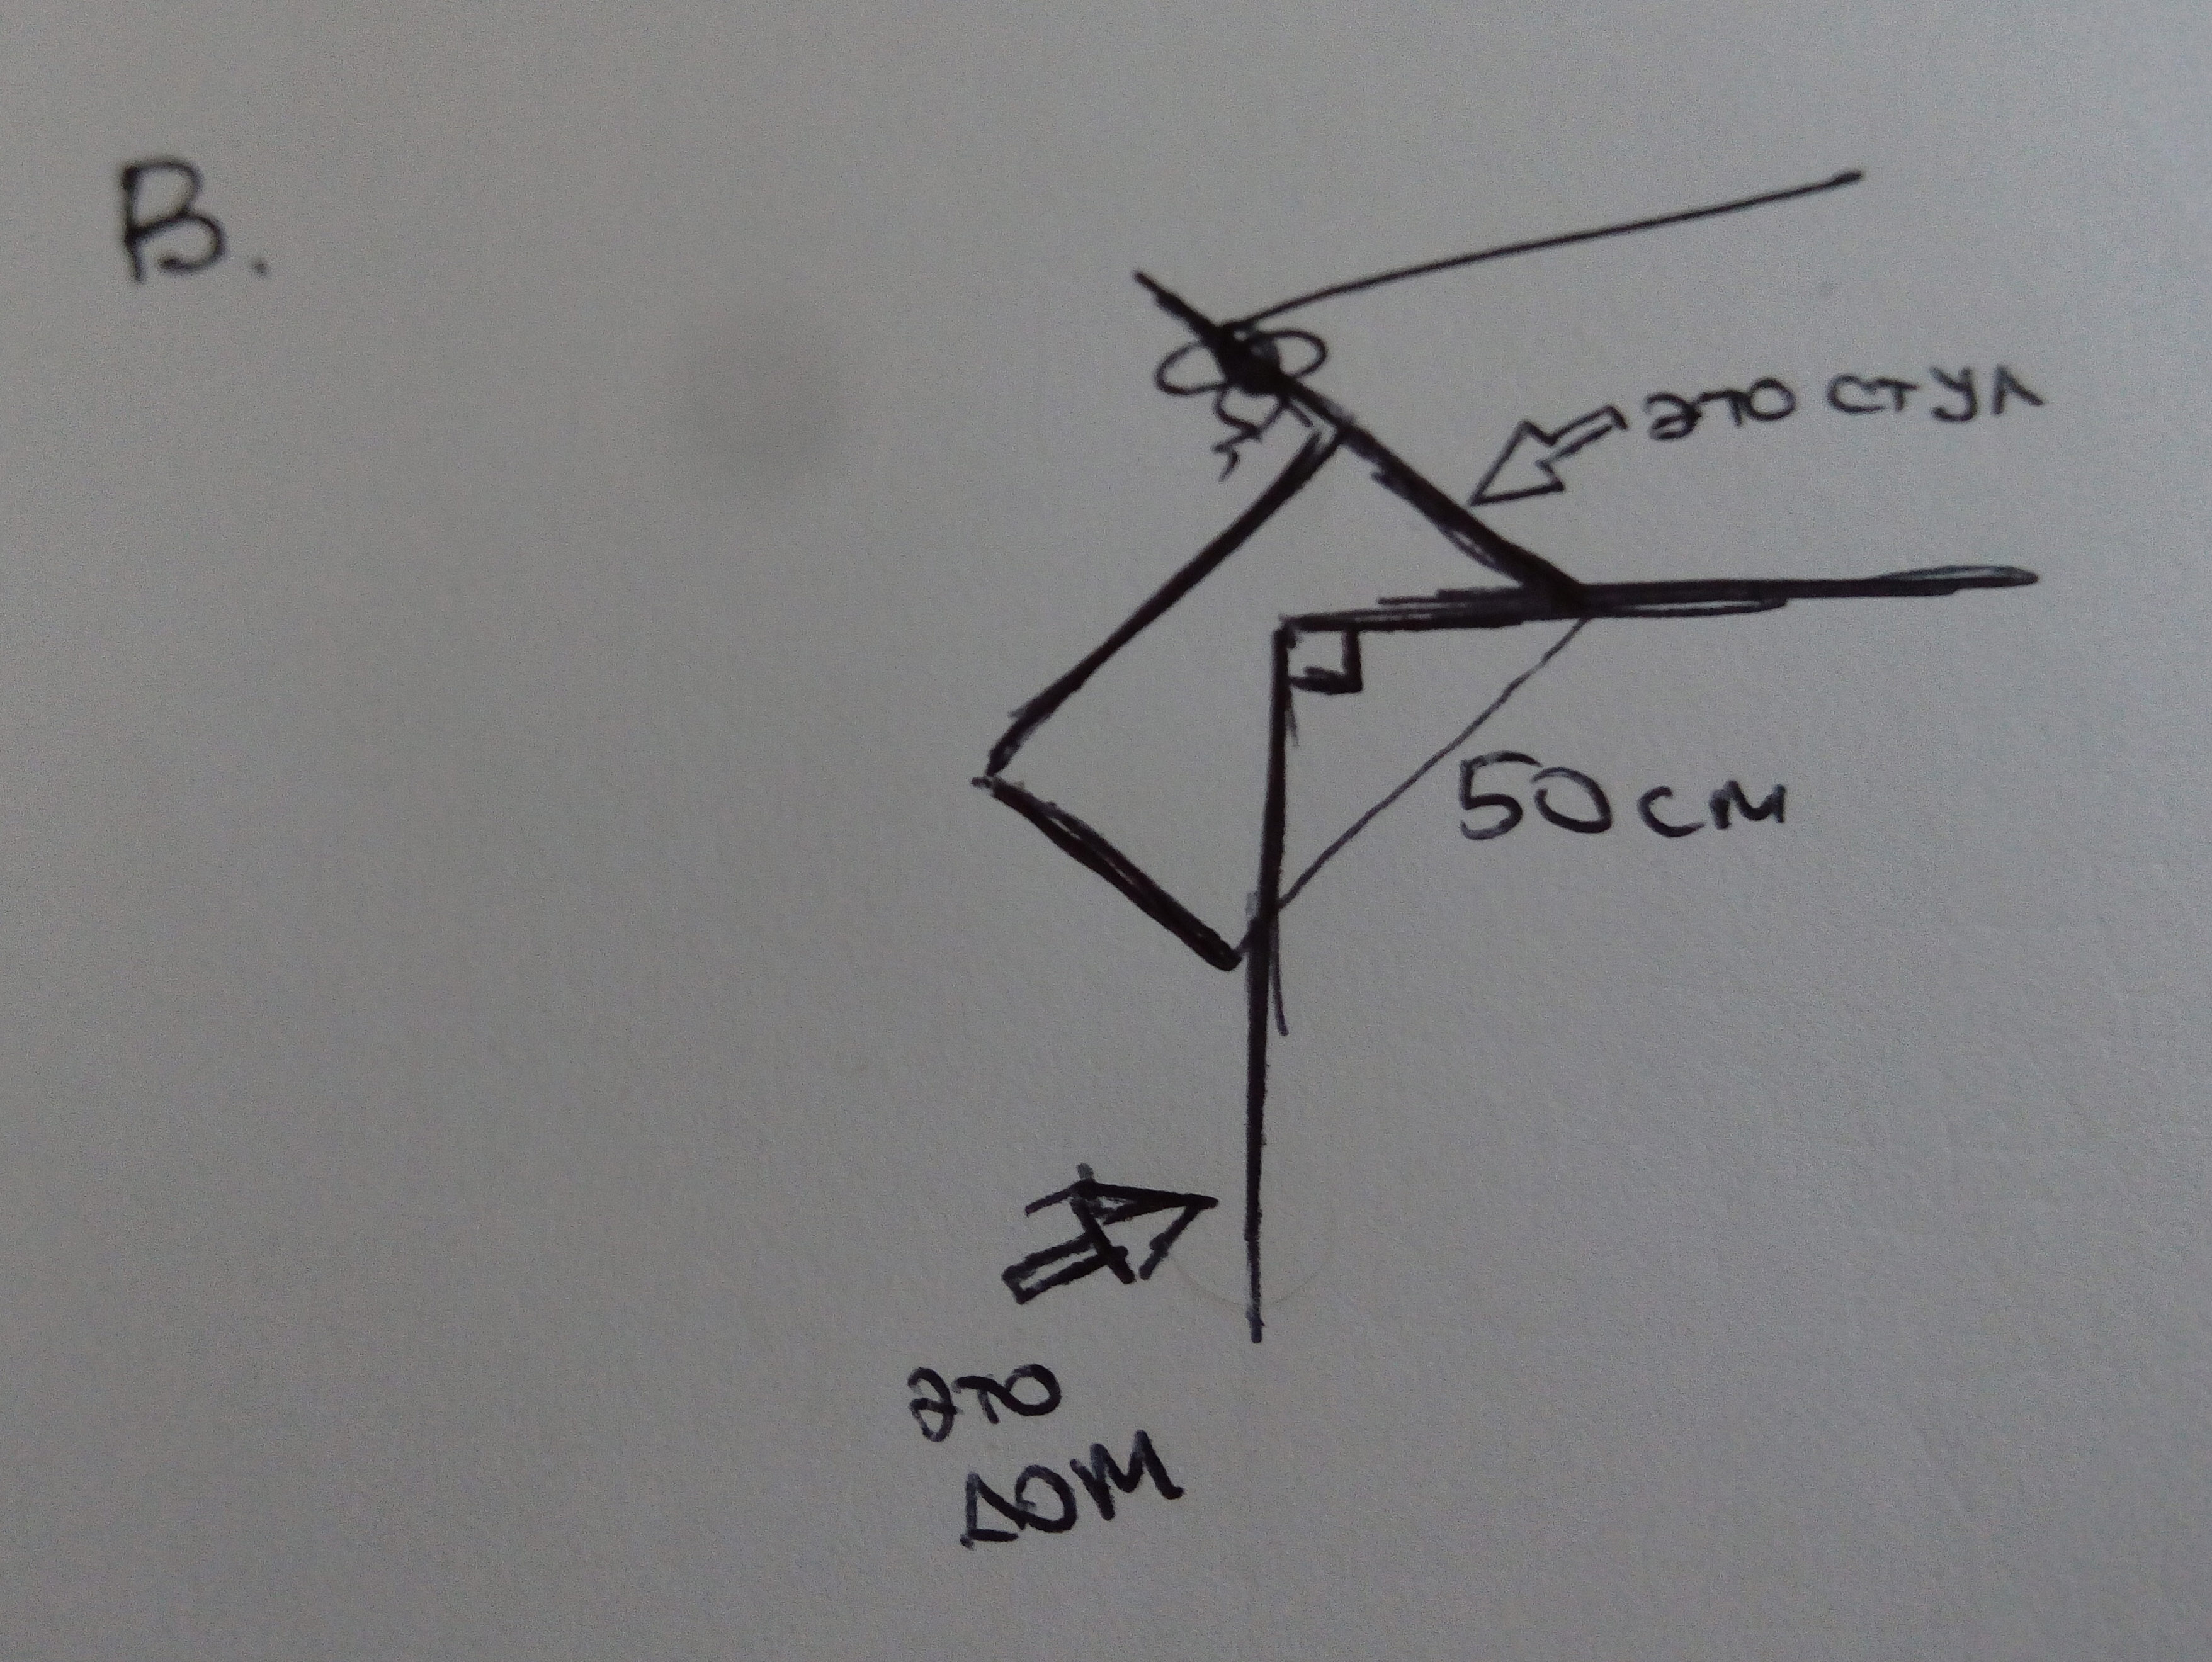
\includegraphics[natwidth=3513,natheight=2640,width=6cm]{figures/2018-clearances-b}
\end{center}

\itC Автобус с диаметром колёс 1 метр и колёсной базой $10.5$ метров (так называют расстояние между передней осью и задней) стоит на планете Маленького принца, диаметр которой 20 метров. Каким должен быть дорожный просвет (расстояние от пола до земли) у автобуса, чтобы он не царапал днищем грунт?

Треугольник, образованный центром планеты и центрами колёс автобуса,~— равносторонний со стороной \SI{10.5}{\text{см}}: одна из сторон равна колёсной базе, а две других~— сумме радиуса планеты (10 метров) и радиуса колеса (0.5 метра).

\begin{center}
	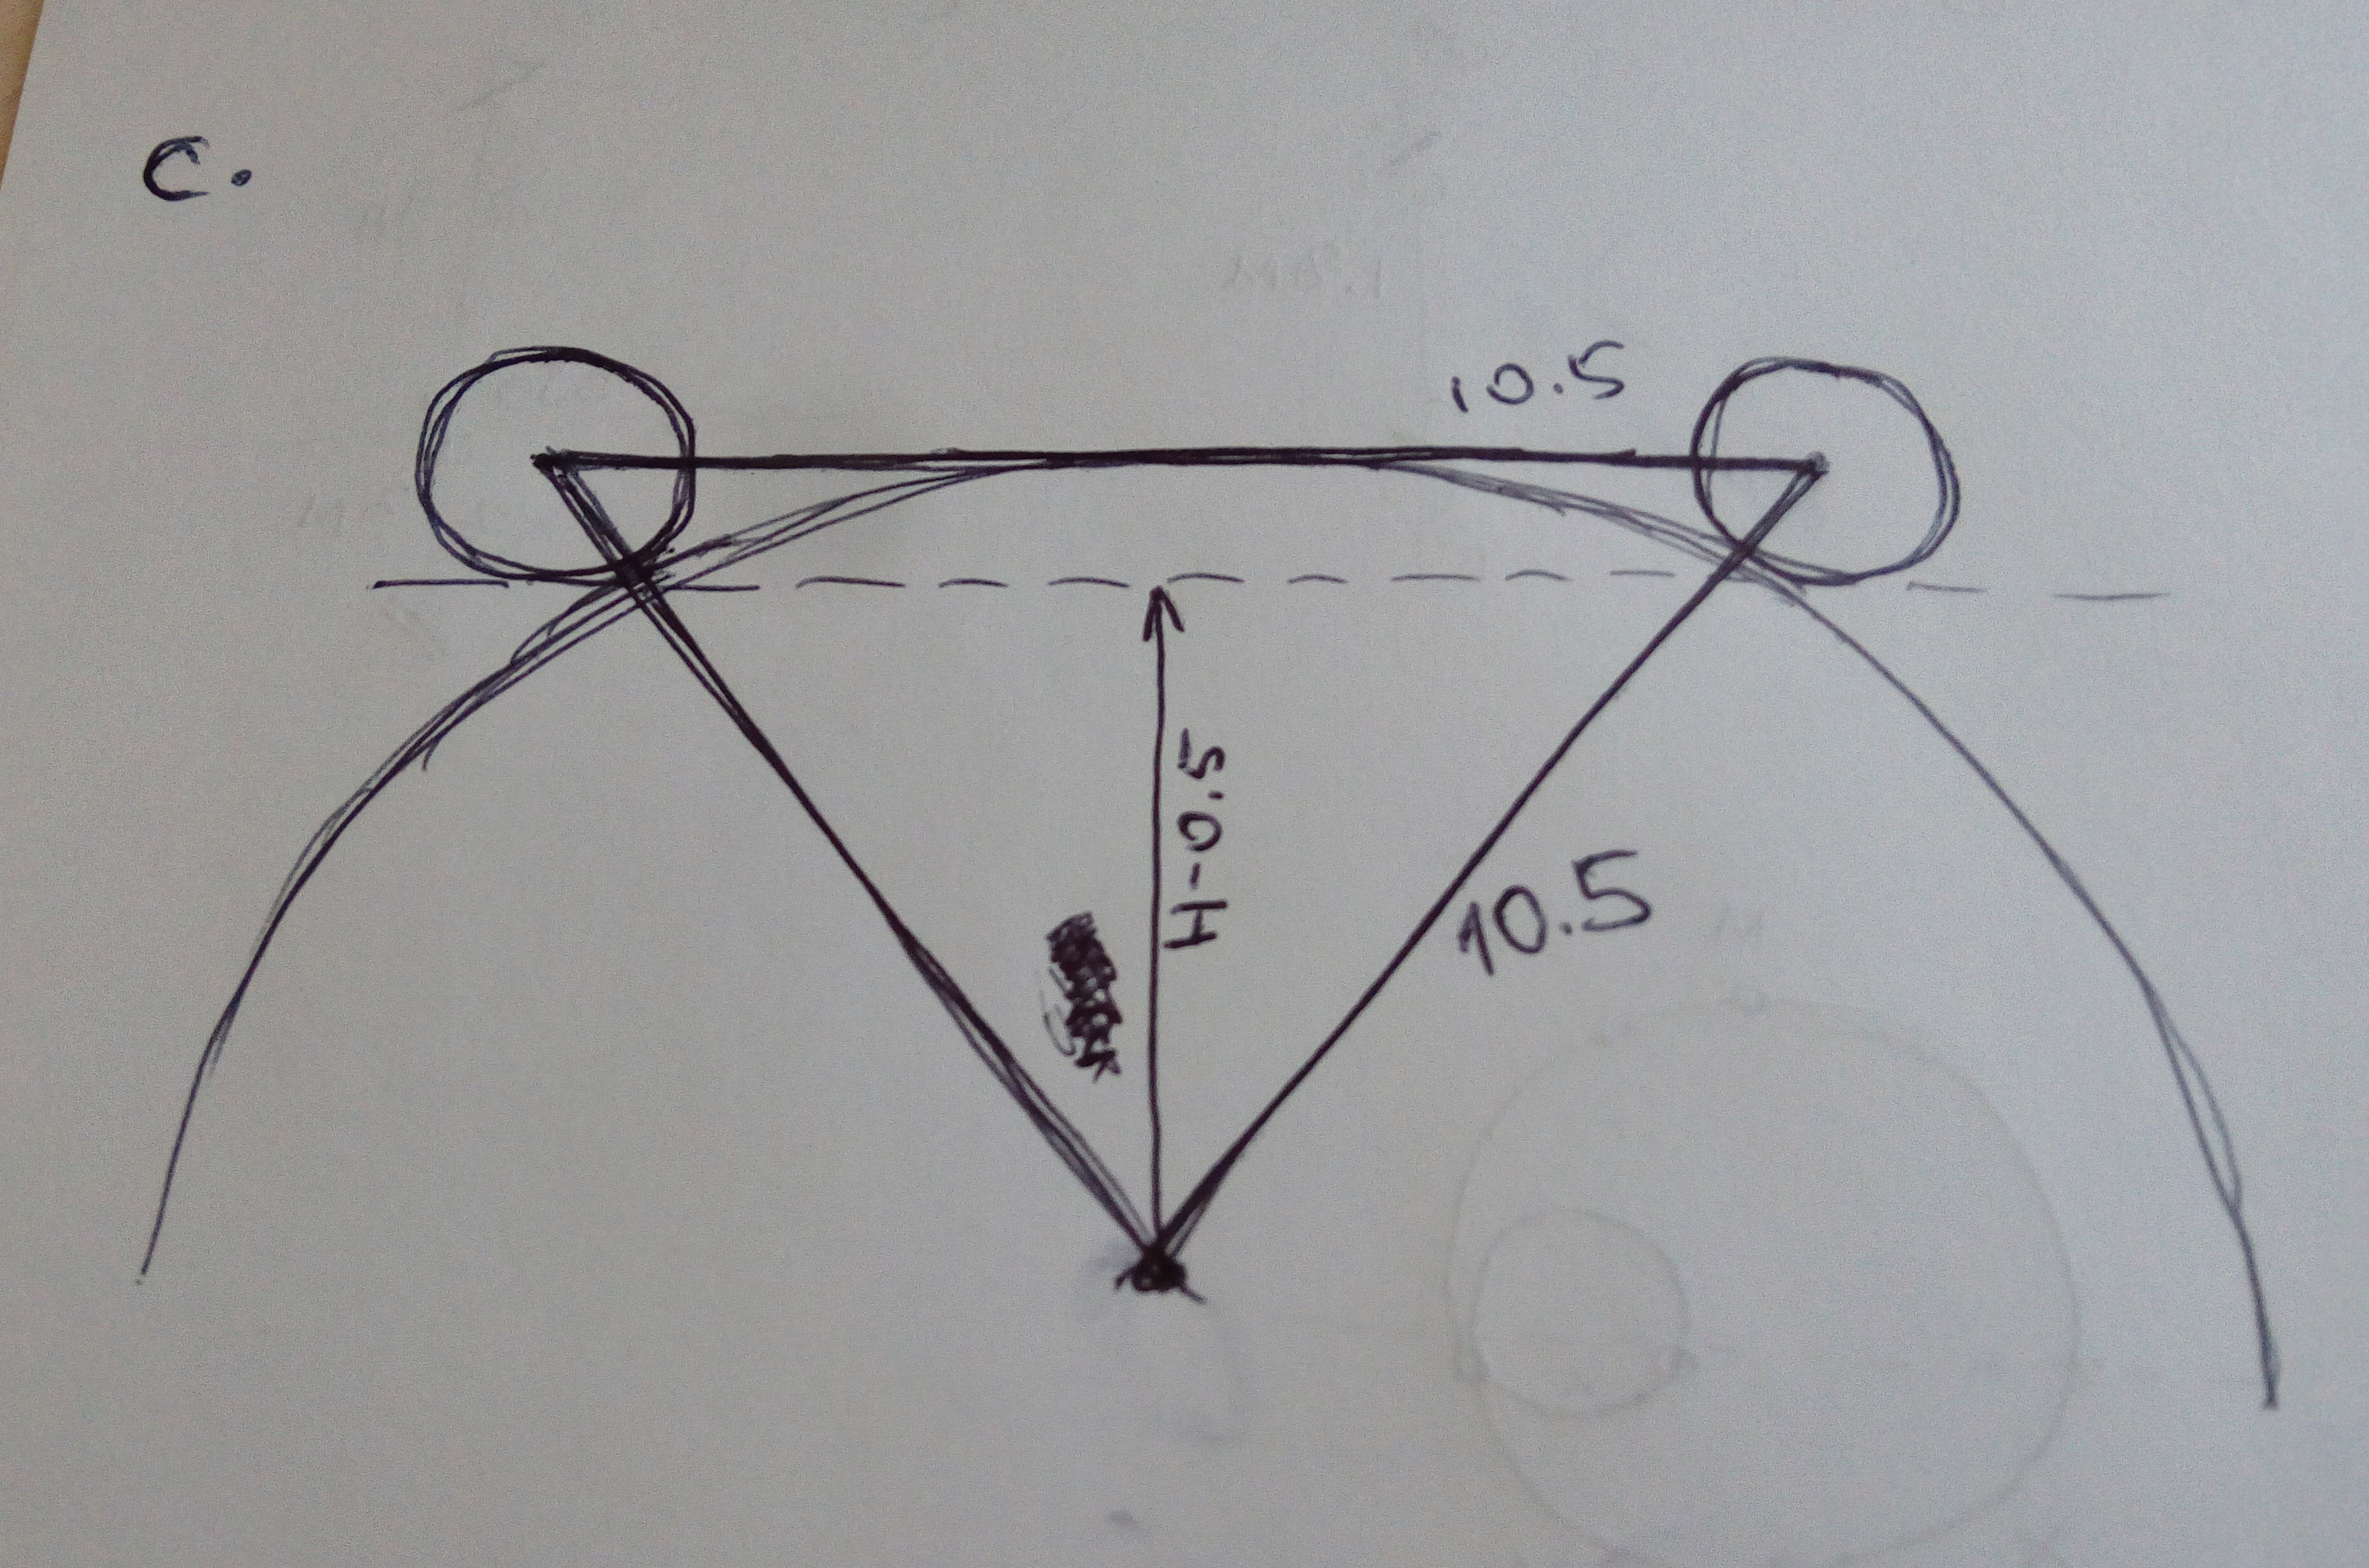
\includegraphics[natwidth=3716,natheight=2460,width=6cm]{figures/2018-clearances-c}
\end{center}

Дорожный просвет автобуса~— расстояние от его пола (который должен касаться верхней точки планеты) до прямой, соединяющей нижние точки колёс. В нашем случае~— это разность $R-(H-0.5)$, где $H$~— высота равностороннего треугольника, а $0.5$~— радиус колеса.

\begin{align*}
	& H = 10.5 \cdot \frac{\sqrt{3}}{2} \\
	& R-(H-0.5) = 11 - 10.5\frac{\sqrt{3}}{2}. \\
	& \text{(это примерно 1.9 метра)}
\end{align*}

Это и есть ответ на задачу.
\end{itemize}